% 勒让德多项式

\section{勒让德多项式}%
\begin{equation}
  \laplacian \varphi = 0
\end{equation}
由 \cref{eq:广义曲线坐标系拉普拉斯算子} 写出求坐标系的拉普拉斯算子,
\begin{equation}
  \laplacian = 
  \frac{1}{r^2} \pdv{r} r^2 \pdv{r} +
  \frac{1}{r^2} \pdv{\theta} \sin \theta \pdv{\theta} +
  \frac{1}{r^2 \sin \theta} \pdv[2]{\phi}
  \label{eq:球坐标系的拉普拉斯算子}
\end{equation}
当函数$\varphi(r, \theta)$与\(\phi\)无关的时候
\begin{equation}
  \begin{aligned}
    \laplacian &= 
  \frac{1}{r^2} \pdv{r} r^2 \pdv{r} +
  \frac{1}{r^2 \sin\theta} \pdv{\theta} \sin \theta \pdv{\theta} +
  \frac{1}{r^2 \sin \theta} \pdv[2]{\phi} \\
\text{(当函数$\varphi(r, \theta)$与\(\phi\)无关的时候)}
\quad &=
  \frac{1}{r^2} \pdv{r} r^2 \pdv{r} +
  \frac{1}{r^2 \sin\theta} \pdv{\theta} \sin \theta \pdv{\theta}
  \end{aligned}
\end{equation}
\begin{equation}
  \begin{aligned}
   & \left(\cancel{\frac{1}{r^2}} \pdv{r} r^2 \pdv{r} +
  \frac{1}{\cancel{r^2} \sin\theta} \pdv{\theta} \sin \theta \pdv{\theta}\right)
  \varphi \\
  &=
  \left(\pdv{r} r^2 \pdv{r} +
  \frac{1}{\sin\theta} \pdv{\theta} \sin \theta \pdv{\theta}\right)
  \varphi = 0
  \end{aligned}
\end{equation}
若 \(\varphi(r, \theta) = R(r) \Theta(\theta)\)
\begin{equation}
 \frac{1}{R} \red{\left(\pdv{r} r^2 \pdv{r} \right) }R=
-\frac{1}{\Theta} \blue{\left(\frac{1}{\sin\theta} \pdv{\theta} \sin \theta \pdv{\theta}\right)} \Theta
  = \lambda
\end{equation}
\begin{align}
  \red{\left(\dv{r} r^2 \dv{r} \right) } R = \lambda R \label{eq:Legendre_R}\\
\blue{\left(\frac{1}{\sin\theta} \dv{\theta} \sin \theta \dv{\theta}\right)}\Theta =  - \lambda \Theta \label{eq:Legendre_Q}
\end{align}
\cref{eq:Legendre_R} 即
\begin{equation}
  \red{\left(\dv{r} r^2 \dv{r} \right) } R = \lambda R 
\end{equation}
的 $r> 0$ 而指数函数\(e^t>0, t\in \RR\),不妨设\(r=e^t\)。
由于
链式法则
\begin{equation}
  \begin{aligned}
  &\dv{f}{r}= \dv{t}{r} \dv{f}{t} = \frac{1}{r} \dv{f}{t} \\
  \implies &\dv{r}=\frac{1}{r} \dv{t}
  \end{aligned}
\end{equation}
得
\begin{equation}
  \red{\left(\dv{r} r^2 \dv{r} \right) } R=
\frac{1}{r} \dv{t} r^2 \frac{1}{r} \dv{t} R
=
\frac{1}{r} \dv{t} r\dv{t} R
= \frac{1}{r} \left( r \ddot{R} + r \dot{R} \right) = \lambda R
\end{equation}
\begin{equation}
\ddot{R} + \dot{R} - \lambda R = 0
\end{equation}
目前\footnote{后面可知,只有当\(l\)为整数时,才能截断}\(\lambda \in \RR\),不妨设\(\lambda = l(l+1), l \in \RR\),
解得
\begin{subequations}
  \begin{align}
  &R_1 = C_1 e^{lt} = C_1 r^l \\
  &R_2 = C_2 e^{(-l-1)t} = C_2 r^{-l-1}
\end{align}
\end{subequations}
\cref{eq:Legendre_Q}做变换, \(x = \cos \theta, \Theta(\theta) \to y=y(x) \)
\begin{equation}
  \blue{\left( \dv{\cos \theta} \sin[2](\theta) \dv{\cos \theta} \right)} \Theta =
  \dv{x} (1-x^2) \dv{x} y = - l(l+1) y
\end{equation}
\begin{equation}
  (1-x^2) \dv[2]{y}{x} - 2 x \dv{y}{x} + l(l+1)y = 0
\end{equation}
在 \(x=0 \quad (\theta= \frac{\pi}{2})\) 处泰勒展开
\begin{equation}
  y=\sum_{k=0}^\infty C_k x^k
\end{equation}
将级数代入勒让德方程,对比系数可以求出
\begin{equation}
  \begin{aligned}
    C_2 &= - \frac{l(l+1)}{2} C_0  \\
        &= - \frac{(l-0)(l+1)}{2} C_0
  \end{aligned}
\end{equation}
\begin{equation}
  \begin{aligned}
    C_3&= -\frac{l(l+1) -2 \cdot 1 }{3 \cdot 2} C_1 \\
&= -\frac{(l-1)(l+2)}{3 \cdot 2} C_1
  \end{aligned}
\end{equation}
\begin{equation}
  \begin{aligned}
    C_{k+2} &= - \frac{(l+1)l - (k+1)k}{(k+2)(k+1)} C_k \quad (k>2)\\
            &= - \frac{(l-k)(l+k+1)}{(k+2)(k+1)} C_k  \qq{(因式分解\footnotemark)}
  \end{aligned}
\end{equation}
综合上式可知
\begin{equation}
    C_{k+2} = - \frac{(l-k)(l+k+1)}{(k+2)(k+1)} C_k  \quad (k\geq 0)
\end{equation}
\footnotetext{\((l-k)(l+k+1) = (l+1)l - (k+1)k\)}
当\(l=0\)时\(C_0=1\),当\(l=1\)时,\(C_0=0,C_1=1\),之后由系数的递推公式可写出系数的通项公式。
当且仅当\(l=0,1,2\dots\)时,系数可被截断。
当\(k\)为偶数的时候,奇数项系数就不能被截断;
当\(k\)为奇数的时候,偶数项系数就不能被截断。
这就要求\(C_0=1\)时,\(C_1=0\);
而\(C_1=1\)时,\(C_0=0\)。
当\(l\)给定后,勒让德方程的解形式上为(注意到有些系数为\(0\))
\begin{equation}
  y = P_l(x) = C_0 + C_1 x + \sum_{k=0}^l C_{k+2} x^{k+2}
\end{equation}
\begin{remark}
  了解一个级数解需要了解
  \begin{itemize}
    \item 母函数
    \item 正交归一性
    \item 递推公式
    \item 通项公式
  \end{itemize}
\end{remark}
\begin{equation}
  \begin{aligned}
    P_l(x) &= \sum_{n}^l \frac{1}{(n!)^2} \frac{\Gamma(l+n+1)}{\Gamma(l-n+1)} \left(\frac{x - 1}{2}\right)^n \\
&= \sum_{n}^l \frac{1}{(n!)^2} \frac{(l+n)!}{(l-n)!} \left(\frac{x - 1}{2}\right)^n
  \end{aligned}
\end{equation}
\begin{equation*}
	\begin{aligned}
		P_l(x) &= \frac{1}{2^l} \sum_{n=0}^{[\frac{l}{2}]}
	(-1)^n \mathrm{C}_l^n \mathrm{C}_{2l - 2n}^{l} x^{l - 2n}\\
&= \frac{1}{2^l} \sum_{n=0}^{[\frac{l}{2}]}
	(-1)^n \frac{(2l - 2n)!}{n! (l-n)! (l-2n)!} x^{l-2n}
	\end{aligned}
\end{equation*}
其中\([\ ]\)代表向下取整
\begin{equation*}
	\left[\frac{l}{2}\right] = 
	\begin{cases}
		\frac{l}{2} & \qq{\(l\) is even } \\
		\frac{l-1}{2} & \qq{\(l\) is odd }
	\end{cases}
\end{equation*}
这两种表示是等价的,见\href{/home/junyi/Documents/Wolfram Mathematica/勒让德多项式.nb}{Mathematica Notebook} 
\begin{align*}
	P_0 = 1 \\
	P_1 = x \\
	P_2 = \frac{1}{2}(3x^2 - 1) \\
	P_3 = \frac{1}{2}(5x^3 - 3x)
\end{align*}
最终拉普拉斯方程的通解可以写作
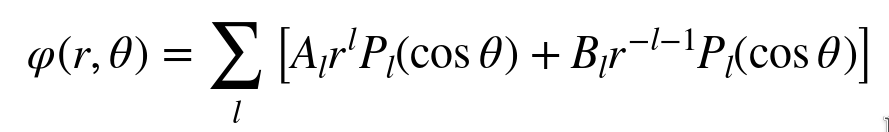
\includegraphics[width=0.5\textwidth]{figures/2022-11-23T222754+0800.png}





%%% vim: set ts=2 sts=2 sw=2 isk+=\: et cc=+1 formatoptions+=mM:
